\clearpage
\section{Konklusjon}

Som vi har vist har lognormal-modellen bedre punktprediksjon enn NB-modellen,
men det kan like gjerne være  overvekt av 0-verdier som gjør punktprediksjonene
bedre. Som nevnt tidligere vil en modell som predikerer verdier rundt 0 ha lav
feil når mesteparten av verdiene er 0 verdier. Her blir det en byttehandel hvor
man får bedre punktprediksjoner, men hvor man har introdusert en skjevhet på
estimatene av modell-parametrene. Dette ser man i PIT-diagrammet i
\cref{fig:PIT_plot}. Vi ser muligens at modellens betingede prediktive
fordelinger ikke egner seg til å beskrive de observerte verdiene. Den
prediktive fordelingen kan bli veldig smal. Dette ser man særlig når andelen 0
verdier er høye (se \cref{fig:pred_plot}, Chad). At lognormal-modellen får
problemer med høye 0-verdier understøttes også at den får høyere DSS-score og
standardisert feil når andelen 0-verdier øker (\cref{fig:p0_plot}). 

NB-modellen er man er bedre kalibrert enn lognormal-modellen. Dette går fram
fra PIT-plottet i \cref{fig:PIT_plot}. Selv om punktprediksjonen er dårligere,
er NB-modellen bedre til å estimere den betingede prediksjonsfordelingen. Dette
trenger vi for å få svar på spørsmål som "hva er sannsynligheten for at det
forekommer tap av menneskeliv i neste uke ($\mathrm{P(Y_{i,t+1} > 0|
Y_{i,t})}$)?". 

I denne undersøkelsen har vi brukt en relativt enkel modell som kun betinger på
antall dødsfall ved uke $t-1$. Begge modellene får problemer med å takle
overgang fra ingen dødsfall en uke til mange den neste uken. Hvis andel
0-verdier er høy vil en No-change modell typisk ha lav feil. Videre er
parametrene estimert ut fra hele tidsserien, noe som tilsvarer en antagelse om
at parametrene ikke endrer gjennom den observerte perioden. Det er mulig at
modellene hadde gjort det bedre ved å legge større vekt på observasjoner som
er nærmere i tid. Man kan tenke seg at man estimerer parametrene kun på
observasjoner fra en måned, et halvår eller år tilbake.

Disse enkle modellene gir gir grunnlag for å utforske negativ
binomial-fordelingen og lognormal-fordelingen videre. En retning som kunne være
av interesse er å tilpasse AR-modeller av høyere orden. Dette er modeller
som ikke bare betinger på den foregående uken, men kan betinge på flere uker i
forkant. En annen retning som kan være av interesse er å sammenligne de to
fordelingene oppfører seg når prediksjonen går over korter eller lengre
tidsintervall. I \cref{fig:monthly_res_plot} vises de standardiserte
residualene for de samme modellene, men hvor ukentlige dødsfall er byttet ut
med månedlige dødsfall. Her ser man spesielt for Chad at det er mindre
forskjell mellom modellene enn når man ser på ukentlige data
(\cref{fig:residuals_orig}).

\begin{figure}[!h]
\centering
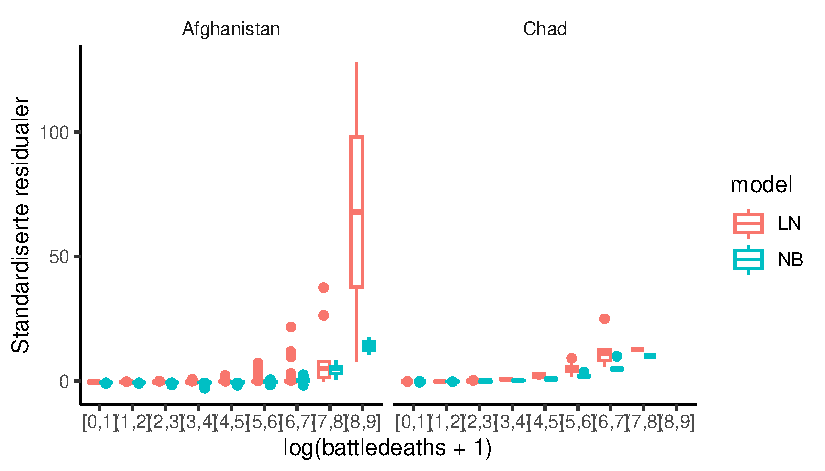
\includegraphics{../img/monthly_res_plot.pdf}
\caption{
    Månedlige log(dødsfall + 1) og standardiserte residualer for Afghanistan og
    Chad.
} 
\label{fig:monthly_res_plot}
\end{figure}


Vi har vist at lognormalfordelingen kan brukes til å få et punktestimat av
antall dødsfall, selv om den prediktive fordelingen ikke beskriver de
observerte dataene. Vi har også vist at negativ binomialfordelingen er mer
fleksibel når man skal modellere data med overspredning og overvekt av
0-verdier.  Vi har og vist at data med stor andel 0-verdier er utfordrende å
modellere. Tidsseriemodellene får problemer når andelene 0-verdier er store.
Når det gjelder punktestimat er vanskelig å utkonkurrere veldig enkel modeller
som NC-modellen (No Change). Det kan være interessant å utforske hvordan de to
fordelingen oppfører seg når perioden man ønsker å predikere for er enten
større eller mindre enn en uke. Videre kan man undersøke hvordan fordelingene
oppfører seg når de brukes sammen med modeller som betinger på flere variabler




